%!TEX TS-program = pdflatex
%!TEX encoding = UTF-8 Unicode

\documentclass[12pt,a4paper,oneside,english,italian]{book}

\usepackage[utf8]{inputenc}

\usepackage{extensions/uniudtesi}

\usepackage[nottoc]{tocbibind}
\usepackage{babel}[italian]
\usepackage{indentfirst}
\usepackage{scalerel}
\usepackage[ruled,vlined,linesnumbered]{algorithm2e}

\graphicspath{{./figure/}}
\usepackage{amsmath,amsfonts,amssymb,amsthm}
\usepackage{latexsym}
\usepackage{graphicx} % [demo] is just for the example
\usepackage{wrapfig}
\usepackage{mathabx}
\usepackage{cancel}[makeroom]

\newcommand{\N}{\mathbb{N}}
\newcommand{\Z}{\mathbb{Z}}
\newcommand{\Q}{\mathbb{Q}}
\newcommand{\R}{\mathbb{R}}
\newcommand{\C}{\mathbb{C}}

% IR functions
\newcommand{\sco}{\text{score}}
\newcommand{\tf}{\text{tf}}
\newcommand{\tfp}{\text{tf}_p}
\newcommand{\idf}{\text{idf}}
\newcommand{\rc}{\text{rc}}
\newcommand{\rel}{\text{rel}}
\newcommand{\re}{\text{R}}
\newcommand{\preci}{\mathcal{P}}


\DeclareMathOperator{\traccia}{tr}
\DeclareMathOperator{\sen}{sen}
\DeclareMathOperator{\arcsen}{arcsen}
\DeclareMathOperator*{\maxlim}{max\,lim}
\DeclareMathOperator*{\minlim}{min\,lim}
\DeclareMathOperator*{\deepinf}{\phantom{\makebox[0pt]{p}}inf}

\newcommand{\varsum}[3]{\sum_{#2}^{#3}\!
   {\vphantom{\sum}}_{#1}\;}
\newcommand{\varprod}[3]{\sum_{#2}^{#3}\!
   {\vphantom{\sum}}_{#1}\;}
\newcommand*{\tokenbox}[1]{\framebox{#1}}

%%%%%%%%%%%%%%%%%%%%%%%%%%%%%%%%%%%%%%%%%%%%%%%%%%%%%%%%%%%

\theoremstyle{plain}
\newtheorem{teorema}{Teorema}[chapter]
\newtheorem{proposizione}[teorema]{Proposizione}
\newtheorem{lemma}[teorema]{Lemma}
\newtheorem{corollario}[teorema]{Corollario}

\theoremstyle{definition}
\newtheorem{definizione}[teorema]{Definizione}
\newtheorem{esempio}[teorema]{Esempio}
\newtheorem{problema}[teorema]{Problema}

\theoremstyle{remark}
\newtheorem{osservazione}[teorema]{Osservazione}

\newcommand{\fsamp}{\textsc{F-samp}\xspace}
\newcommand{\base}{\textsc{base}\xspace}
\newcommand{\fcount}{\textsc{F-count}\xspace}


\usepackage{makeidx}
\makeindex

% Ridefiniamo la riga di testa delle pagine:
\usepackage{fancyhdr}
\pagestyle{fancy}
\renewcommand{\chaptermark}[1]{\markboth{#1}{}}
\renewcommand{\sectionmark}[1]{\markright{\thesection\ #1}}
\fancyhf{}
\fancyhead[LE,RO]{\bfseries\thepage}
\fancyhead[LO]{\bfseries\rightmark}
\fancyhead[RE]{\bfseries\leftmark}
\renewcommand{\headrulewidth}{0.5pt}
\renewcommand{\footrulewidth}{0pt}
\setlength{\headheight}{14.5pt}

  \titoloeng{Exploring BM25P\cr hyperparameters space}
  \titolo{Esplorazione dello spazio degli iperparametri di BM25P}
  \laureando{Federico Silvestri}
  \annoaccademico{2019-2020}
  %\facolta{Scienze Matematiche, Fisiche e Naturali}
  \corsodilaureatriennalein{Informatica}
  \relatore[Prof.]{Maria Simi}
  \relatoreDue[Dott.]{Cristina Ioana Muntean}
  \dedica{Dedicato alle persone più care che ho incontrato \\ e che tuttora, anche se in modo diverso, \\ sono con me. }

% Per l'ipertesto:
 \usepackage{hyperref} % gia' caricato da uniudtesi
 \hypersetup{
  bookmarksopen, % default
  bookmarksopenlevel=2, % default;
  pdftitle={Exploring BM25P hyperparameter space},
  pdfauthor={Federico Silvestri},
  pdfsubject={Thesis of Bachelor Degree in Computer Science},
  pdfkeywords={Thesis Bachelor Degree Computer Science Federico Silvestri}
  }
  
\usepackage{listings}
\usepackage{xcolor}
\definecolor{listinggray}{gray}{0.9}
\definecolor{lbcolor}{rgb}{0.9,0.9,0.9}
\lstset{
	backgroundcolor=\color{lbcolor},
	tabsize=2,    
	language=Java,
	basicstyle=\scriptsize,
	upquote=true,
	aboveskip={1.5\baselineskip},
	columns=fixed,
	showstringspaces=false,
	extendedchars=false,
	breaklines=true,
	prebreak = \raisebox{0ex}[0ex][0ex]{\ensuremath{\hookleftarrow}},
	frame=single,
	numbers=left,
	showtabs=false,
	showspaces=false,
	showstringspaces=false,
	identifierstyle=\ttfamily,
	keywordstyle=\color[rgb]{0,0,1},
	commentstyle=\color[rgb]{0.026,0.112,0.095},
	stringstyle=\color[rgb]{0.627,0.126,0.941},
	numberstyle=\color[rgb]{0.205, 0.142, 0.73},
}

 \lstset{
 	backgroundcolor=\color{lbcolor},
 	tabsize=2,
 	language=Java,
 	captionpos=b,
 	tabsize=2,
 	frame=lines,
 	numbers=left,
 	numberstyle=\tiny,
 	numbersep=5pt,
 	breaklines=true,
 	showstringspaces=false,
 	basicstyle=\footnotesize,
 	% identifierstyle=\color{magenta},
 	keywordstyle=\color[rgb]{0,0,1},
 	commentstyle=\color[rgb]{0,0.39,0},
 	stringstyle=\color{red},
 	morecomment=[l][\color{magenta}]{\#}
 }


\usepackage{bold-extra}
\usepackage{lmodern}

\begin{document}
\nocite{*}
\renewcommand{\theequation}{\thechapter.\arabic{equation}}
\renewcommand{\thesection}{\thechapter.\arabic{section}}

\frontmatter

\maketitle

\cleardoublepage

\tableofcontents

% \listoffigures

\mainmatter

% \let\cleardoublepage\clearpage
 
 \chapter{Descrizione del tirocinio}

Il tirocinio si è svolto quasi sempre in modalità telematica,
sia perché la situazione dovuta al COVID-19 non ha concesso
gli spostamenti, sia perché  il lavoro che doveva essere svolto
era per lo più individuale.
Sono stato supervisionato principalmente da tre persone,
le quali mi hanno dato degli obiettivi da raggiungere per ogni
step del tirocinio,
fino ad arrivare alla conclusione.
Il codice implementato risiede in piccola
quantità nell'appendice di questa relazione,
e invece tutto il progetto e tutte le sperimentazioni
sono disponibili sulla pagina personale di \href{https://github.com/federicosilvestri/bm25p-thesis}{GitHub}.

Il tirocinio si è concluso una volta raggiunti i risultati
previsti, e le ore totali impiegate sono state circa 320.

\subsection{Basi di partenza}
Questo tipo di tirocinio si è basato
sullo studio di una materia non trattata nel corso di laurea triennale:
\textit{Information Retrieval} (\textit{IR}).
Tale materia è risultata abbastanza facile da comprendere grazie
al materiale fornito dai tutor e alla loro disponibilità.
Una volta approfondito lo studio è iniziata la fase sperimentale,
cioè la progettazione e l'implementazione di svariati meccanismi per la ricerca 
degli iperparametri ottimi di BM25P.

L'algoritmo BM25P è un'estensione della funzione di ranking
di BM25, un noto algoritmo nel ramo dell'\textit{IR}.
BM25P è stato ideato e pubblicato su ACM dal C.N.R.
stesso nel 2019.\cite{10.1145/3331184.3331373}

Per verificare la validità di ciò che è stato trovato
si sono utilizzati dei test statistici, di cui l'articolo\cite{10.1145/1321440.1321528}
ha consigliato.

Per concludere si sono verificate alcune ipotesi
che erano state fatte dai tutor come premessa
del tirocinio stesso.

\subsection{Linguaggi utilizzati}
I linguaggi che sono stati utilizzati sono stati prevalentemente Java e Python.
Java è stato utilizzato per estendere le funzionalità della piattaforma Terrier,
mentre Python per eseguire alcuni esperimenti statistici.
Non sono mancate anche le competenze di scrittura di script
bash e di amministrazione di sistemi Linux, sui quali sono stati
eseguiti gli esperimenti prodotti.

\subsection{Ambienti di sviluppo}
Per sviluppare l'estensione di Terrier sono stati utilizzati principalmente
l'Ambiente di Sviluppo Integrato \textit{IntelliJ} e \textit{Maven},
come gestore dei pacchetti di Java, che
è lo standard adottato dalla piattaforma.
Per la ricerca e la sperimentazione è stato fatto uso di Jupyter Notebook
e Matlab, che si sono rivelati utili per la presentazione dei grafici
e dei test statistici.

 
\chapter{Introduzione}
Al giorno d'oggi cercare informazioni sul web è diventata una delle operazioni più comuni e più richieste:
utilizzare lo smartphone per eseguire una ricerca sui punti di interesse di una città, o per scoprire la ricetta di un dolce è capitato quasi a tutte le persone.
Le statistiche elaborate direttamente da Google affermano che ogni secondo vengono richieste circa \textit{40.000} query, per un totale
giornaliero di \textit{3,5 miliardi}.
Siamo arrivati persino a parlare di memoria \textit{transattiva}, ovvero di una memoria condivisa tra tutti gli utenti e disponibile attraverso il web.
Infatti l'essere umano che possiede un qualunque mezzo tecnologico è in grado di accedervi in svariati modi, per esempio facendo una ricerca tramite Siri, Google oppure Alexa.
Tale memoria non consiste nel memorizzare l'informazione stessa, ma in come giungere ad essa.
Ma non è solo all'interno del web che c'è la necessità di un sistema di ricerca. Si pensi per esempio a Spotlight di Mac OS, dove
viene utilizzato  per file di testo, audio, immagini e anche news dalla rete.
Il ruolo dell'Information Retrieval in questi giorni è dunque di fondamentale importanza.
Per questo gli algoritmi si sono dovuti sviluppare in tutte le dimensioni: a partire dall'architettura delle macchine sulle quali i documenti vengono archiviati a come i documenti stessi vengono strutturati. In questa tesi di tirocinio verrà illustrato \textit{Terrier}, una piattaforma sviluppata dall'università di Glasgow
per sperimentare gli algoritmi legati all'Information Retrieval, anche su collezioni di dati nell'ordine dei terabyte.  Successivamente il focus si sposterà
sugli algoritmi di ranking, dei quali andremo a utilizzare BM25P, una versione di BM25 migliorata dal gruppo ISTI del CNR di Pisa.
Verranno illustrati una serie di algoritmi il cui scopo è quello di ricercare, all'interno di uno spazio multidimensionale,
gli \textit{iperparametri} di BM25P, incrementando dunque le prestazioni rispetto a BM25 stesso.
Attraverso dei test statistici verificheremo infine che i due modelli di ranking sono decisamente diversi ed è possibile
inferire in quali \textit{passages} sono contenute le informazioni più \textit{rilevanti}, in forte relazione al tipo di collezione di documenti.

\section{Architettura generale}
In questo capitolo verrà illustrata l'architettura generale di un sistema di IR e verranno
descritti alcuni processi che sono stati oggetto di studio del tirocinio.
Quando si parla di sistema di IR, oppure in termini più quotidiani di \textit{search engine},
siamo spesso abituati a vederlo come un sistema di interrogazione dove l'utente
digita come input un testo, chiamato query e il motore risponde con una serie di risultati. Tali risultati
sono visualizzati all'utente come una lista di documenti che contengono informazioni
rilevanti secondo la query.
\`E immediato pensare all'esempio di Google, dove l'utente digita una serie di termini
all'interno del  form e dopo qualche secondo gli vengono restituiti tutti i link a pagine web che
sono in qualche modo collegate a ciò che l'utente stava realmente cercando.
Quello che sta dietro a tutto questo processo, che sembra essere quasi immediato nell'esempio di Google, è
in realtà un lavoro molto complesso e lungo.
La fase che l'utente è abituato ad esserne partecipe è la fase finale, ovvero
il \textit{Retrieving}. Ma prima di poter parlare di ciò è necessario illustrare la fase primaria, l'\textit{Indexing}.

\paragraph{Alcune definizioni}
Per essere più chiari, conveniamo alcune definizioni di termini tecnici che al giorno d'oggi possono essere attribuiti
a concetti diversi.

\begin{definizione}\label{def:token}
	Un token è un'istanza di una sequenza di caratteri, in un documento $d \in \mathcal{D}$, che
	sono raggruppati tra di loro come un'unità semanticalmente utile.
\end{definizione}

\begin{esempio}[tokenizzazione]
	Nella frase "Nulla si crea, nulla si distrugge ma tutto si trasforma" i token sono i seguenti:
	\tokenbox{nulla} \tokenbox{si} \tokenbox{crea} \tokenbox{nulla} \tokenbox{si} \tokenbox{distrugge}
	\tokenbox{ma} \tokenbox{tutto} \tokenbox{si} \tokenbox{trasforma}.
\end{esempio}

Un altro concetto importante è il concetto di tipo.
\begin{definizione}[tipo]\label{def:tipo}
	Un tipo è una classe di token con la solita sequenza di caratteri.
\end{definizione}
\begin{esempio}
	Consideriamo la frase dell'esempio precedente. I tipi sono 7, mentre i token sono 10. Abbiamo dunque
	3 token che si ripetono.
\end{esempio}
\begin{definizione}[query]\label{def:query}
	Una query è un multinsieme di token, che rappresenta l'input che il motore di ricerca
	riceve dall'utente. 
\end{definizione}
Da notare che il concetto di multinsieme deriva dal fatto che si vuole tenere traccia in modo esplicito 
della molteplicità
dei termini nella query stessa.

\begin{definizione}[termine]\label{def:temine}
	Un termine è un tipo di una query.
\end{definizione}

\paragraph{Fase di indexing}
Per poter offrire quella velocità che si richiede durante la fase di retrieving è necessario aver ``preparato"
una struttura dati che sia completa, ovvero che comprenda tutte le informazioni necessarie, e 
rapida da scorrere, ovvero che le informazioni che si stanno cercando devono poter essere recuperate
il prima possibile.  Un esempio abbastanza esplicativo è quello dell'addetto alla biblioteca che deve rispondere
alle richieste degli studenti. Se l'addetto non conoscesse i libri che sono parte della biblioteca, per ogni richiesta
dovrebbe scorrere tutta la lista e capire se quel dato libro può essere utile oppure no.
Questo esempio rappresenta il fatto che l'addetto non è in possesso di una struttura in grado
di accedere solo alle informazioni necessarie ed è dunque inefficiente.
Se quindi non ci fosse un indice, per un motore di ricerca sarebbe troppo dispendioso elaborare tutti
i documenti "su richiesta".
La fase di indexing ha lo scopo di costruire una struttura dati, chiamata indice, che consenta
di velocizzare la fase successiva, il Retrieving.
Dal punto di vista delle prestazioni tale fase è quella con il  dispendio computazionale
più elevato, sia in termini di spazio che di tempo.
Questo perché si devono analizzare tutti i documenti della collezione ed eseguire una serie di elaborazioni
su di essi.
Il seguente algoritmo illustra in modo abbastanza basico ma intuitivo, la funzione eseguita dall'indexer.
\begin{algorithm}[h]
	\small
	\DontPrintSemicolon
	\SetKwInOut{Input}{Input}
	\SetKwInOut{Output}{Output}
	\Input{$\mathcal{D} $ collezione di documenti}
	\Output{$\mathcal{I}$ indice}
	\BlankLine
	$\mathcal{I} = generateEmptyIndex()$\;
	\ForEach{$d \in \mathcal{D}$}{
		$tokenizer = getTokenizer(d)$\;
		\While{$token = tokenizer.nextToken()$}{
			$n = normalizeToken(token)$\;
			$updateIndex(\mathcal{I}, n, d)$\;
		}
	}
	\Return{$\mathcal{I}$}
	\caption{\textsc{}}
	\label{alg:indexing}
\end{algorithm}
L'idea alla base è quella di rappresentare un documento come un flusso di token, il che è sempre possibile
poiché conveniamo che in questo campo di information retrieval i documenti sono solo di tipo testuale.
Il token prima di essere passato alla funzione $updateIndex$ viene normalizzato. La normalizzazione è un processo
che si occupa di risolvere alcuni problemi legati al riconoscere quando due token sintanticamente diversi
hanno invece la solita semantica\footnote{Potrebbe essere necessario uno step in più per risolvere il problema della codifica, poiché alcune lingue posseggono caratteri che non tutte le codifiche hanno. Per esempio le
	lingue cirillica e cinese.}
Tale processo può essere schematizzato nel seguente modo, dove a sinistra viene indicato
il nome della normalizzazione e a destra una breve descrizione.
\begin{itemize}
	\item[Casing] le lettere maiuscole vengono convertite in minuscole
	\item[Accenti] le parole con accenti vengono convertite in parole senza accenti
	\item[Stemming] i verbi vengono convertiti in una forma normale, per esempio nel tempo infinito.
	\item[Lemmization] le parole plurali vengono convertite in singolari
\end{itemize}

\begin{esempio}[normalization]
	Sia data la seguente frase: ``\textit{Mi piacciono tutte le auto che sono elettriche}".
	Utilizzando le tecniche elencate in precedenza, i token normalizzati risultano:
	\tokenbox{Mi} \tokenbox{piacere} \tokenbox{tutte} \tokenbox{le} \tokenbox{auto}
	\tokenbox{che} \tokenbox{essere} \tokenbox{elettriche}.
\end{esempio}

\subparagraph{Indice invertito}
Una volta normalizzato si procede all'aggiornamento dell'indice, ovvero alla costruzione (o aggiornamento)
dell'indice invertito. Tale struttura è definita come una lista di coppie
$\langle token, PostingList \rangle$ dove PostingList è una lista di \textit{identificatori di documenti}.
In questo modo possiamo sapere il token $x$ in quali documenti è contenuto, cercando dentro l'indice
invertito la posizione di $x$ e accedendo alla sua \textit{postingList}.

\begin{figure}[h]
	\label{fig:invertedIndex}
	\centering
	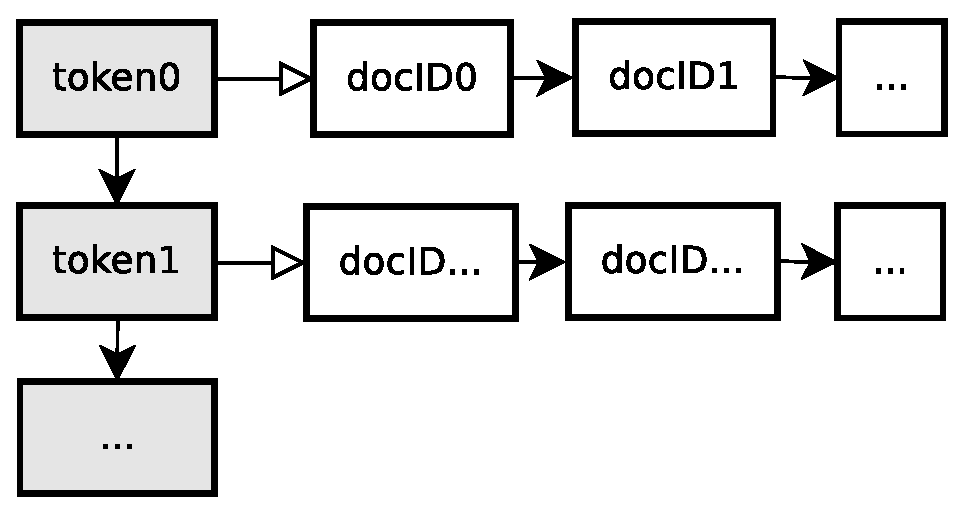
\includegraphics[scale=0.4]{InvertedIndex.eps}
\end{figure}

Ritornando all'esempio della biblioteca, se l'addetto avesse a disposizione l'indice invertito potrebbe:
\begin{enumerate}
	\item Raccogliere la query $\mathcal{Q}$ dello studente
	\item Normalizzare $\mathcal{Q}$
	\item $\forall t.t\in Q$ cercare all'interno dell'indice invertito il termine $t$ e \textit{ritornare} la \textit{postingList} associata
\end{enumerate}

In questo modo tutti i documenti che contengono almeno una volta un termine della query verrebbero mostrati
agli studenti, ma ovviamente non tutti possono essere rilevanti per la ricerca. Il problema dunque si ridotto
a come utilizzare l'indice invertito per capire quanto la query sia associata al documento in questione, ed è per questo
motivo che viene introdotta la fase di \textit{Retrieve}

\paragraph{Fase di Retrieving}
Lo scopo della fase di retrieving è quello di utilizzare l'indice invertito e affinare il modo con cui
i documenti vengono proposti all'utente, comunemente chiamati \textit{risultati}.
Tale processo prende anche il nome di ranking, poiché l'idea alla base è quella di attribuire
un punteggio ad ogni risultato e costruire una lista ordinata in senso crescente.
Ovviamente il primo risultato è quello secondo cui il sistema di ranking è più
rilevante per la query $q$. Tale processo viene fatto ogni volta che l'utente
interroga il sistema, per cui deve essere veloce, efficiente ed effettivo.
L'articolo \cite{10.1016/j.ipm.2016.05.004} mostra una serie di tecniche che possono essere
utilizzate per valutare il tradeoff tra qualità di un ranker ed efficienza, di cui alcune
sono state utilizzate nell'ambito di questo tirocinio.\\
Per essere più precisi possibile, possiamo definire la funzione di score nel seguente modo

\begin{definizione}\label{def:funzione_di_score_ideale}
	Una funzione di scoring $f(d,q) : \mathcal{D} \times \mathcal{Q} \rightarrow \mathbb{R}$ è tale
	se e solo se:
	\begin{itemize}
		\item $f(d_1,q_1) \geq f(d_2, q_2) \implies \rel(d_1, q_1) \geq \rel(d_2, q_2)$,\\ dove $\rel(d,q)$ è la rilevanza del documento $d$ per la query $q$, calcolata a priori.
		\item $f(d,q) \leq 0$ significa che il documento è irrilevante per $q$.
	\end{itemize}
\end{definizione}

Tale definizione definisce una funzione di scoring ideale, per la quale non esiste un algoritmo che
la calcoli. Possiamo però accontentarci di funzioni che la approssimano, facendo uso di euristiche basate sulla statistica. \footnote{Solo per revisione: questo è quello che grossomodo credo di aver elaborato e penso che abbia anche una corrispondenza a livello teorico. }
Nei prossimi capitoli verranno descritte le funzioni di scoring che propongono BM25 e BM25P, le quali si basano sul concetto di \textit{Term Frequency} e \textit{Inverse Document Frequency}.
Prima di concludere la visione generale diamo la definizione di alcuni concetti che sono utilizzati durante il retrieving.

\begin{definizione}[Raw Count]\label{def:raw_count}
	$\rc(q, D) : \mathcal{Q} \times \mathcal{D} \rightarrow \mathbb{N}$ è detto raw count, cioè il numero di volte che
	il termine q occore nel documento $d$.
\end{definizione}

\begin{definizione}[Term Frequency]\label{def:}
	La funzione $\tf(q,d)$, acronimo di Term Frequency, è una funzione che calcola la frequenza del
	termine $q \in \mathcal{Q}$ nel documento $d \in \mathcal{D}$.
	Tale valore si discosta da quello di $rc$, poiché solitamente è normalizzato o in scala logaritmica
	oppure in base alla lunghezza del documento.
	
	\begin{itemize}
		\item $\tf(q,d) = \log_{k}(1+\rc(q,d))$ con $k>1$
		\item $\tf(q,d) = \frac{rc(q,d)}{|d|}$ dove $|d|$ è il numero totali di token nel documento
	\end{itemize}
\end{definizione}

\begin{definizione}[Inverse Document Frequency]\label{def:idf}
	$$
	\idf(q, \mathcal{D}) = \log_{k>1}{
		\frac{\#\mathcal{D}}{
			\#
			\left\{
			d \in \mathcal{D} \middle \lvert rc(q,d) > 0
			\right\} 
		}
	}
	$$
	
	Tale misura esprime quanta informazione una parola, o più un generale un token, fornisce.
	Si può anche pensare come la misura dalla rarità, cioè quanto è comune il termine $q$
	nella collezione di documenti $\mathcal{D}$.
\end{definizione}





 
\section{Architettura generale}
In questo capitolo verrà illustrata l'architettura generale di un sistema di IR e verranno
descritti alcuni processi che sono stati oggetto di studio del tirocinio.
Quando si parla di sistema di IR, oppure in termini più quotidiani di \textit{search engine},
siamo spesso abituati a vederlo come un sistema di interrogazione dove l'utente
digita come input un testo, chiamato query e il motore risponde con una serie di risultati. Tali risultati
sono visualizzati all'utente come una lista di documenti che contengono informazioni
rilevanti secondo la query.
\`E immediato pensare all'esempio di Google, dove l'utente digita una serie di termini
all'interno del  form e dopo qualche secondo gli vengono restituiti tutti i link a pagine web che
sono in qualche modo collegate a ciò che l'utente stava realmente cercando.
Quello che sta dietro a tutto questo processo, che sembra essere quasi immediato nell'esempio di Google, è
in realtà un lavoro molto complesso e lungo.
La fase che l'utente è abituato ad esserne partecipe è la fase finale, ovvero
il \textit{Retrieving}. Ma prima di poter parlare di ciò è necessario illustrare la fase primaria, l'\textit{Indexing}.

\paragraph{Alcune definizioni}
Per essere più chiari, conveniamo alcune definizioni di termini tecnici che al giorno d'oggi possono essere attribuiti
a concetti diversi.

\begin{definizione}\label{def:token}
	Un token è un'istanza di una sequenza di caratteri, in un documento $d \in \mathcal{D}$, che
	sono raggruppati tra di loro come un'unità semanticalmente utile.
\end{definizione}

\begin{esempio}[tokenizzazione]
	Nella frase "Nulla si crea, nulla si distrugge ma tutto si trasforma" i token sono i seguenti:
	\tokenbox{nulla} \tokenbox{si} \tokenbox{crea} \tokenbox{nulla} \tokenbox{si} \tokenbox{distrugge}
	\tokenbox{ma} \tokenbox{tutto} \tokenbox{si} \tokenbox{trasforma}.
\end{esempio}

Un altro concetto importante è il concetto di tipo.
\begin{definizione}[tipo]\label{def:tipo}
	Un tipo è una classe di token con la solita sequenza di caratteri.
\end{definizione}
\begin{esempio}
	Consideriamo la frase dell'esempio precedente. I tipi sono 7, mentre i token sono 10. Abbiamo dunque
	3 token che si ripetono.
\end{esempio}
\begin{definizione}[query]\label{def:query}
	Una query è un multinsieme di token, che rappresenta l'input che il motore di ricerca
	riceve dall'utente. 
\end{definizione}
Da notare che il concetto di multinsieme deriva dal fatto che si vuole tenere traccia in modo esplicito 
della molteplicità
dei termini nella query stessa.

\begin{definizione}[termine]\label{def:temine}
	Un termine è un tipo di una query.
\end{definizione}



\paragraph{Fase di indexing}
Per poter offrire quella velocità che si richiede durante la fase di retrieving è necessario aver ``preparato"
una struttura dati che sia completa, ovvero che comprenda tutte le informazioni necessarie, e 
rapida da scorrere, ovvero che le informazioni che si stanno cercando devono poter essere recuperate
il prima possibile.  Un esempio abbastanza esplicativo è quello dell'addetto alla biblioteca che deve rispondere
alle richieste degli studenti. Se l'addetto non conoscesse i libri che sono parte della biblioteca, per ogni richiesta
dovrebbe scorrere tutta la lista e capire se quel dato libro può essere utile oppure no.
Questo esempio rappresenta il fatto che l'addetto non è in possesso di una struttura in grado
di accedere solo alle informazioni necessarie ed è dunque inefficiente.
Se quindi non ci fosse un indice, per un motore di ricerca sarebbe troppo dispendioso elaborare tutti
i documenti "su richiesta".
La fase di indexing ha lo scopo di costruire una struttura dati, chiamata indice, che consenta
di velocizzare la fase successiva, il Retrieving.
Dal punto di vista delle prestazioni tale fase è quella con il  dispendio computazionale
più elevato, sia in termini di spazio che di tempo.
Questo perché si devono analizzare tutti i documenti della collezione ed eseguire una serie di elaborazioni
su di essi.
Il seguente algoritmo illustra in modo abbastanza basico ma intuitivo, la funzione eseguita dall'indexer.
\begin{algorithm}[h]
	\small
	\DontPrintSemicolon
	\SetKwInOut{Input}{Input}
	\SetKwInOut{Output}{Output}
	\Input{$\mathcal{D} $ collezione di documenti}
	\Output{$\mathcal{I}$ indice}
	\BlankLine
	$\mathcal{I} = generateEmptyIndex()$\;
	\ForEach{$d \in \mathcal{D}$}{
		$tokenizer = getTokenizer(d)$\;
		\While{$token = tokenizer.nextToken()$}{
			$n = normalizeToken(token)$\;
			$updateIndex(\mathcal{I}, n, d)$\;
		}
	}
	\Return{$\mathcal{I}$}
	\caption{\textsc{}}
	\label{alg:bray-curtis}
	
\end{algorithm}
L'idea alla base è quella di rappresentare un documento come un flusso di token, il che è sempre possibile
poiché conveniamo che in questo campo di information retrieval i documenti sono solo di tipo testuale.
Il token prima di essere passato alla funzione $updateIndex$ viene normalizzato. La normalizzazione è un processo
che si occupa di risolvere alcuni problemi legati al riconoscere quando due token sintanticamente diversi
hanno invece la solita semantica\footnote{Potrebbe essere necessario uno step in più per risolvere il problema della codifica, poiché alcune lingue posseggono caratteri che non tutte le codifiche hanno. Per esempio le
lingue cirillica e cinese.}
Tale processo può essere schematizzato nel seguente modo, dove a sinistra viene indicato
il nome della normalizzazione e a destra una breve descrizione.
\begin{itemize}
	\item[Casing] le lettere maiuscole vengono convertite in minuscole
	\item[Accenti] le parole con accenti vengono convertite in parole senza accenti
	\item[Stemming] i verbi vengono convertiti in una forma normale, per esempio nel tempo infinito.
	\item[Lemmization] le parole plurali vengono convertite in singolari
\end{itemize}

\begin{esempio}[normalization]
	Sia data la seguente frase: ``\textit{Mi piacciono tutte le auto che sono elettriche}".
	Utilizzando le tecniche elencate in precedenza, i token normalizzati risultano:
	\tokenbox{Mi} \tokenbox{piacere} \tokenbox{tutte} \tokenbox{le} \tokenbox{auto}
	\tokenbox{che} \tokenbox{essere} \tokenbox{elettriche}.
\end{esempio}

Una volta normalizzato si procede all'aggiornamento dell'indice, ovvero nella costruzione
dell'\textit{indice invertito}. 
 
\chapter{Metriche}

In questo capitolo si  illustreranno alcune tecniche 
per valutare un modello di pesi e dunque poterlo confrontare con gli altri.
\'E di necessaria importanza poterlo fare perché nel capitolo sull'ottimizzazione di BM25P dovremo avere un modo per eseguire
la cosidetta fase di \textit{model selection}. Dovremo cioè valutare se un modello con un iperparametro $\lambda$ è
migliore rispetto a un modello con un iperparametro $\lambda' \neq \lambda$.

Ma in generale per valutare le prestazioni di un motore di ricerca possiamo usare due unità di misura:

\begin{itemize}
	\item La \textbf{qualità}, intesa come l'effettività, cioè quanto il motore di ricerca
	è in grado di mostrare all'utente documenti che siano rilevanti con la query $q$.
	\item L'\textbf{efficienza}, cioè quanto tempo viene impiegato nel calcolo dei risultati, quindi in questo caso
	quanto tempo impiega la fase di \textit{retrieval}.
\end{itemize}

L'obiettivo di questo tirocinio è stato quello di massimizzare la qualità di BM25P, pertanto
la seconda unità di misura non è rilevante, anche perché variando il valore di un iperparametro
non si hanno ripercussioni notevoli sull'efficienza, ma solo sulla qualità.

Per poter valutare l'effettività è necessario riprendere il concetto di rilevanza  che era stato
accennato nel capitolo 1. Essa purtroppo è una misura non del tutto oggettiva,
poiché un utente potrebbe decidere che la query $q$ e il documento $d$ siano
in qualche modo collegati tra loro o meno.

\begin{esempio}
	Sia $q$ la query \textit{``python"}. L'utente potrebbe intendere sia il linguaggio di programmazione Python
	che l'animale stesso. Dunque se questa query fosse sottomessa a un motore di ricerca
	esso potrebbe ritornare al fruitore entrambi i risultati, che a seconda della necessità
	potrebbe valutarli come rilevanti oppure no.
\end{esempio}

Ciò che l'utente intende è chiamata \textit{Information Need}, cioè la richiesta di informazione
che si tenta di esprimere sottomettendo una query al sistema di ricerca.

La soggettività di questa valutazione è uno dei punti cruciali dell'Information Retrieval, per cui non esistono
metodi matematici per calcolarla ed è necessario l'intervento umano.
Viene enunciata dunque la definizione di rilevanza booleana:

\begin{definizione}\label{def:relb}
	La rilevanza booleana $\rel_B(d,q): \mathcal{D} \times \mathcal{Q} \rightarrow \mathbb{B}$
	è una funzione binaria che associa alla coppia query-documento un valore booleano
	true o false, in questo modo:
	\begin{itemize}
		\item		$\rel_B(d,q) = true$ se e solo se l'utente ritiene che il documento d è rilevante
		per la query $q$.
		\item $\rel_B(d,q) = false$ altrimenti.
	\end{itemize}
	
	Anche se ovvio, sottolineamo il fatto che $\rel_B(q,d)$ dipende unicamente dalla query q e
	dal documento $d$. In altri contesti questo concetto può esser chiamato anche con il nome
	di \textit{ground truth} oppure \textit{gold standard}.
\end{definizione}

Il valore di tale funzione deve sempre esser calcolato da un essere umano, poiché come da definizione, 
deve rappresentare una verità soggettiva.

Ciò potrebbe sembrare però un po' limitante, poiché quando si parla di scoring,
$\sco(q,d)$ restituisce valori continui in $\mathbb{R}$ e dunque come può
approssimare $\rel_B$?
La risposta sta nel fatto che un ranker $\mathcal{R}$ si limita ad ordinare i documenti utilizzando come peso
il valore attribuito al documento dalla funzione $\sco$. Pertanto se ipotizzassimo di prendere
i primi $k$ elementi dalla lista $\mathcal{L}$, restituita dal motore di ricerca, potremo affermare che:

\begin{itemize}
	\item Se $d \in \mathcal{L}$  allora $\rel_{\mathcal{R}}(d, q) = true$
	\item Se $d \notin \mathcal{L}$ allora $\rel_{\mathcal{R}}(d,q) = false$
\end{itemize}

Attraverso questa definizione siamo in grado dunque di stabilire le modalità di valutazione di
un motore di ricerca, poiché possiamo paragonare i risultati di $\rel_B$ con quelli di $\rel_{\mathcal{R}}$,
ottenendo dunque un meccanismo di comparazione tra i risultati attesi e quelli calcolati.

\subsection{Il principio PRP}

In questo paragrafo viene introdotto il \textit{Probability Ranking Principle}, ovvero un risultato
teorico che ci consenta di avere una base matematica per valutare l'ottimalità di un ranker.
Tale principio afferma che:

\begin{definizione}\label{def:prp}
	Se per ogni query $q \in \mathcal{Q}$ il sistema ordina i documenti della collezione $\mathcal{D}$ in
	senso decrescente rispetto alla probabilità di rilevanza, allora l'effettività complessiva del sistema
	è la migliore ottenibile con i dati a disposizione.
\end{definizione}

Questo principio rappresenta l'unico metodo formale per verificare l'effettività di un sistema
di ricerca, poichè migliore è la stima della rilevanza, migliori saranno le prestazioni.

Per completezza della trattazione dell'argomento verrà data di seguito
un'illustrazione di come dimostrare questo principio.

\begin{proof}
	Iniziamo la dimostrazione procedendo per punti:
	\begin{itemize}
		\item Sia $\mathcal{R}$ un ranker
		\item Siano $\mathcal{Q}$ e $\mathcal{D}$ gli insiemi delle query e dei documenti
		\item In questo contesto, sia $\rel_\mathcal{R}$ una variabile con natura aleatoria
		\item $\forall{q \in \mathcal{Q}, d \in \mathcal{D}}$ sia $P(\rel_B = r  | D = d, Q = q )$
		la probabilità che il documento $d$ sia rilevante per $q$.
		\item Sia $\mathcal{L}$  la lista ordinata dei documenti ritornati dal motore di ricerca, di lunghezza arbitraria
		$k$.
	\end{itemize}
	
	Il valore atteso della rilevanza possiamo calcolarlo come:
	\begin{align*}
	& \mathbb{E}\left[\rel_B\right] = \sum_{i=1}^{k}{
		1 \cdot P(\rel_B = true  | D = d_i, Q = q ) + \cancelto{0}{0 \cdot  P(\rel_B = false  | D = d_i, Q = q )}
	} \\
	& \mathbb{E}\left[\rel_B\right] = \sum_{i=1}^{k}{P(\rel_B = true  | D = d_i, Q = q )}
	\end{align*}
	
	Ciò che vogliamo dimostrare è che per ogni valore di $k>0$, il valore atteso è massimo quando i documenti
	sono ordinati in senso decrescente.
	Procediamo dunque per assurdo ipotizzando esista un valore $\tilde{k}$ tale che $\mathbb{E}[\rel_B]$ sia
	massimo anche se i documenti non sono ordinati in tal modo.
	Si verifica dunque che esiste almeno un documento $d_l$ che non viene inserito in $\mathcal{L}$ nell'ordinamento
	decrescente e inoltre ciò impone che un altro documento $d_m$ non venga inserito nell'ultima posizione della lista.
	Abbiamo quindi che:
	$$
	P(\rel_B = r | D = d_l, Q=q)  < P(\rel_B = r| D = d_m, Q = q)
	$$
	
	e dunque:
	
	\begin{align*}
	& \mathbb{E}\left[\rel_B\right]_{\tilde{k}} = \sum_{i=1}^{\tilde{k}}{P(\rel_B = true | D = d_i, Q = q)} \\
	& \mathbb{E}[\rel_B]_{\tilde{k}} \Big|_{d_{\tilde{k}} = d_{l}} < \mathbb{E}[\rel_B]_{\tilde{k}} \Big|_{d_{\tilde{k}} = d_{m}}
	\end{align*}
	
	Ciò però è assurdo, perché per ipotesi $\mathbb{E}\left[\rel_B\right]_{\tilde{k}}$ sostituendo $d_{\tilde{k}}$ con $d_l$ doveva
	essere massimo.
\end{proof}

\section{Recall e Precision}

Adesso che abbiamo raccolto tutte le informazioni necessarie possiamo definire
le unità di misura che descrivono la qualità di un motore di ricerca.
Le misure più semplici che sono adottate attualmente sono  la \textit{recall} e la \textit{precision}.

\begin{definizione}\label{def:recall}
	La recall, indicata con il simbolo $\re$, è definita come il rapporto tra il numero di documenti
	messi in lista da  un ranker $\mathcal{R}$, per cui $\rel_B(d,q) = true$,
	e il numero di elementi totali giudicati rilevanti.
	In simboli si ha:
	
	$$
	\re = P(d \in \mathcal{L} | \rel_B(d,q) = true) = \frac{
		\#\left\{ d \in \mathcal{L} | \rel_B(d,q) = true\right\}
	}{
		\#\left\{ d \in \mathcal{D} | \rel_B(d,q) = true\right\}
	}
	$$
\end{definizione}

Ovviamente affinchè la recall sia massima, il ranker dovrebbe ritornare la lista di tutti i documenti
rilevanti, ma questo non sempre risulta possibile, poiché $\left|\mathcal{L}\right| \lll \left|\mathcal{D}\right|$.

\begin{definizione}\label{def:precision}
	La precision, indicata con il simbolo $\preci$, è uguale alla recall
	ma con la differenza che il rapporto non ha come denominatore tutti i documenti
	rilevanti, ma solo quelli in lista.
	
	$$
	\re = P(d \in \mathcal{L} | \rel_B(d,q) = true) = \frac{
		\#\left\{ d \in \mathcal{L} | \rel_B(d,q) = true\right\}
	}{
		\left|\mathcal{L}\right|
	}
	$$
\end{definizione}
Invece per precision, raggiungere il valore massimo è abbastanza facile, specialmente quando $\left|\mathcal{L}\right| \approx 1$.

\pagebreak

Un modo analogo per calcolare $\re$ e $\preci$ è quello di creare una sorta di matrice di contingenza, nel seguente modo:

\begin{table}[h!]
	\centering
	\begin{tabular}{|c|c|c|}
		\hline
		& $\rel_b = true$ & $\rel_b = false$ \\
		\hline
		$d \in \mathcal{L}$ &  vero positivo (tp) & falso positivo (fp) \\
		\hline
		$d \notin \mathcal{L}$ &  falso negativo (fn) & vero negativo (tn) \\
		\hline
	\end{tabular}
	\caption{Matrice di contingenza, o matrice di confusione}
\end{table}

Una volta avvalorata la matrice, si può calcolare $\preci = \frac{tp}{tp + fp}$ e $\re = \frac{tp}{tp + fn}$.

\paragraph{Il problema delle misure}
Il problema principale di queste due misure è il fatto che statisticamente il $99.9\%$\cite{irbook} dei documenti
risulta non rilevante per una query $q$. 
Infatti se la funzione obiettivo da massimizzare fosse recall,
un sistema che marca tutti i documenti come non rilevanti avrebbe
un valore molto vicino ad un sistema che invece funziona bene. Inoltre
queste misure sono basate sull'insieme dei documenti restituiti e non tengono
conto dell'ordine della lista $\mathcal{L}$.

Per esempio un utente che naviga nel web è interessato
ad avere come primo risultato esattamente il documento che stava cercando
e non vorrebbe scorrere i risultati fino a trovare quello che gli interessava.
Precision e recall quindi sono misure semplici ed effettive, ma non
complete per la valutazione di un motore di ricerca.

\section{NDCG}
L'unità di misura che andremo a considerare è la Normative Discontinued Cumulative Gain,
definita come segue:

$$\label{def:ndcg}
NDCG(O, k) = \frac{1}{\left|O\right|} \sum_{q \in O} Z_{k, q} \cdot \sum_{i=1}^{k} \frac{2^{R(d_i, q)} - 1}{\log_2{(i + 1)}} \\
$$

in cui abbiamo che:
\begin{table}[h!]
	\centering
	\begin{tabular}{|c|c|}
		\hline
		$ O \subset Q$ & è un sottoinsieme di query \\
		\hline
		$Z_{k,q}$ & è il fattore di normalizzazione \\
		\hline
		$R(d,q)$ & è il gold standard, possiamo assumerla uguale a $\rel_B$ \\
		\hline
	\end{tabular}
\end{table}

Come è possibile notare dalla formula, in questo modo andiamo a considerare un sottoinsieme delle query, che chiamiamo $O$,
e un intero $k>1$ che conta il numero di documenti nella lista $\mathcal{L}$.

Espandendo la seconda sommatoria $s_2$ è interessante notare che:
$$
s_2 = \frac{2^{R(d_1, q) } - 1}{1} + \frac{2^{R(d_2, q)} - 1}{1.58} + \frac{2^{R(d_3, q)} - 1}{2} + \dotsb + \frac{2^{R(d_k, q) } - 1}{\log_2{k + 1}}
$$

Siccome la funzione $log_2(x)$ è monotona crescente, $s_2$ è costruita in modo tale da
premiare maggiormente i risultati con $k$ piccolo e penalizzare quelli con $k$ più grande.
Parlando anche in termini computazionali, calcolare il valore dell'esponente al numeratore
non è troppo dispendioso poiché:

\begin{enumerate}
	\item la base dell'esponente è 2 e il valore di $R(d,q)$ è intero, dunque si può fare bit shifting;
	\item la funzione $R(d,q)$ inoltre, se la ipotizziamo uguale a $\rel_B$ assume solo due valori,
	o anche se fosse diversa essa assumerebbe un insieme finito di valori che può essere precomputato.
\end{enumerate}

La prima parte della formula invece non fa altro che calcolare una media aritmetica
dei singoli valori ottenuti valutando una query. Infatti è possibile semplificarla
nel caso in cui si voglia calcolare la valutazione rimuovendo la prima parte, come verrà fatto
negli esempi successivi.

\begin{esempio}[Calcolo di DCG]\label{eg:dcg}
	Ipotizziamo di calcolare il valore di DCG (NDCG non normalizzata) avendo a disposizione:
	\begin{itemize}
		\item i risultati $\mathcal{L} = \left\{r_1, r_2, r_3, r_4\right\}$, ordinati per rank,
		\item le rilevanze associate ai risultati, cioè $\rel_B\left(\mathcal{L}\right) = \left\{1, 0, 0, 1\right\}$
	\end{itemize}

$$
DCG = \frac{2^{1} - 1}{1} + \frac{2^{0} - 1}{1.58} + \frac{2^{0} - 1}{2} + \frac{2^{1} - 1}{2.32} = 1.43
$$
\end{esempio}

\paragraph{Fattore di normalizzazione}
Al fine di rendere DCG normalizzata, ovvero a valori in $\left[0, 1\right]$, si introduce il fattore di
normalizzazione, chiamato  $Z_{k, q}$. Il pedice $k,q$ indica che esso può dipendere dalla lunghezza
della lista e dalla query.
Un esempio di normalizzazione potrebbe essere quello di usare l'$i$DCG (la $i$ sta per ideale),
cioè il valore di DCG se i risultati fossero ordinati correttamente.

\begin{esempio}\label{eg:ndcg}
	 Per rendere la funzione dell'esempio \ref{eg:dcg}  normalizzata, si può calcolare
	 il fattore $Z_{k,q}$ come segue.
	 L'ordinamento ideale per i documenti potrebbe essere $\mathcal{L}_i = \left\{r_1, r_4, r_3, r_2\right\}$,
	 oppure tutte le permutazioni di esso per cui $\rel_B(\mathcal{L}_i)= \left\{1,1,0,0\right\}$.
	 $$
	 Z_{k,q} = iDCG = \frac{2^{1} - 1}{1} + \frac{2^{1} - 1}{1.58} + \frac{2^{0} - 1}{2} + \frac{2^{0} - 1}{2.32} = 1.63
	 $$
	 
	 dunque NDCG è pari a:
	 $$
	 NDCG = \frac{1.43}{1.63} = 0.88
	 $$
\end{esempio}

Attraverso questa misura abbiamo ottenuto un meccanismo di valutazione che è in grado di tenere in considerazione
sia il problema della quantità di dati, sia quello dell'ordinamento; inoltre  non viene
usato direttamente il valore della funzione di ranking, ma l'ordinamento dei risultati.
Ciò ci consente dunque di essere in grado di valutare qualsiasi motore di ricerca
senza fare restrizioni sulla funzione di ranking.


\chapter{BM25 e BM25P}

\chapter{Ricerca degli iperparametri}

\paragraph{Introduzione}
In questa sezione della relazione verrà illustrato il problema principale affrontato nel tirocinio:
\textit{l'ottimizzazione della funzione di ranking di BM25P}.
Come illustrato nel capitolo 2, quasi ogni funzione di ranking possiede degli iperparametri, i quali
devono essere calibrati a seconda del tipo di dati e dalla natura dei dati stessi.
Per esempio se si dovesse calibrare BM25 per una collezione
di documenti medico-scientifici, esso potrebbe avere degli iperparametri
differenti da quelli adatti per una collezione di documenti esclusivamente matematici.
Questo aspetto rende molto simile il mondo dell'Information Retrieval a quello del Machine Learning,
infatti alcuni termini e concetti sono di comune utilizzo.


Ricapitolando, gli iperparametri di BM25P sono:
\begin{table}[h!]
	\centering
	\begin{tabular}{|c|c|c|}
		\hline
		Parametro & Vincoli & Descrizione \\
		\hline
		$p$ & $p>1$ & numero di passages \\
		\hline
		$\alpha$ & $\alpha > 0$ & costante di amplificazione \\
		\hline
		$\boldsymbol{w}$ & $\forall{i.1 \leq i \leq p}\implies \boldsymbol{w}_i \geq 0$ & vettore dei pesi dei passaggi \\
		\hline
	\end{tabular}
\caption{Iperparametri di BM25P}
\end{table}

Per questioni pratiche, la scelta che si è deciso di fare è quella di cercare
nello spazio dei valori di $\boldsymbol{w}$, poiché esso rappresenta l'iperparametro
che agisce sui passages, che è la particolarità introdotta da BM25P stesso, e lasciare
$p$ e $\alpha$ costanti.

\paragraph{La funzione obiettivo}

Come in qualsiasi ambito di ricerca nello spazio degli stati, anche in questo contesto
si deve scegliere una funzione da massimizzare e vedremo che essa presenterà dei problemi ben
noti i quali limiteranno la scelta dei possibili algoritmi applicabili.

Una delle misure che meglio esprimono l'efficacia di un motore di ricerca è NDCG \ref{def:ndcg}, la quale è
stata illustrata e commentata nel capitolo 4.
Massimizzando questa funzione siamo dunque in grado di ottenere una funzione di ranking che
è ottima per un certo dataset $\mathcal{D}$.

\paragraph{Obiettivo}
L'obiettivo che dunque bisogna porsi è quello di rispondere alle seguenti domande, ipotizzando
di avere $\mathcal{D}$:

\begin{enumerate}
	\item Quali sono gli iperparametri da impostare all'algoritmo per massimizzarne la qualità?
	\item Quali sono gli algoritmi per il calcolo di tali iperparametri?
	\item Di quanto possiamo aumentare l'efficienza di BM25 utilizzando l'estensione dei passages?
	\item Qual è la natura del vettore $\boldsymbol{w}$?
\end{enumerate}

Nei seguenti paragrafi verranno illustrati i meccanismi che sono stati
trovati, implementati e testati e ne verranno forniti anche alcuni risultati
sperimentali. Alla fine della relazione inoltre sono presenti anche alcune
parti del codice Java.

\section{Setup sperimentale}

Una volta concluso lo studio di come Terrier è stato costruito e di come la sua pipeline è stata implementata,
il tirocinio si è focalizzato sulla ricerca di algoritmi adatti a fare \textit{model selection}.

\paragraph{Dataset}
Il dataset fornito insieme a Terrier, chiamato \textit{Vaswani}, è un dataset abbastanza piccolo,
contenente soltanto 10.000 titoli di documenti. Per poter avere dei risultati più
reali è stato utilizzato \textit{Aquaint}, acquistato con licenza dal C.N.R.
Esso contiene circa un milione di documenti e i relativi file di test, quali
un \textit{topic file} di 50 query e il \textit{qrels file} associato.
\textit{Aquaint} è un dataset prodotto da David Graff nel 2002,
contenente un elenco di notizie provenienti da tre fonti principali:
lo Xinhua News Service, il New York Times e l'Associated Press WorldStream News Service.


\paragraph{Macchine a disposizione}
Per poter accedere a tali dati, di dimensioni notevoli, è stato necessario utilizzare
delle macchine specifiche fornite dall'ente stesso, poiché sia per ragioni di sicurezza
che per ragioni pratiche, i dati non potevano essere resi pubblici.
Mi è stato dunque fornito l'accesso ad una macchina 
all'interno della rete del C.N.R. in grado di sostenere il carico
di lavoro che gli algoritmi di ricerca avrebbero potuto richiedere.

\section{La pipeline di ricerca}
Per poter eseguire la massimizzazione della funzione obiettivo,
è necessario eseguire una serie di operazioni, che configurano il sistema Terrier
in modo da poter elaborare i dati con i parametri impostati.
Verrà dato di seguito una lista ordinata delle operazioni da eseguire:

\begin{enumerate}
	\item \textbf{Inizializzare} gli iperparametri scelti ad un valore iniziale.
	\item \textbf{Eseguire} la fase di \textit{recupero}, producendo dunque una serie di risultati.
	\item \textbf{Eseguire} la fase di \textit{evaluation}, calcolando dunque il valore della funzione obiettivo.
	\item \textbf{Confrontare} il valore attuale della funzione obiettivo con quello in memoria.
	\item \textbf{Aggiornare} gli iperparametri e tornare al punto 2.
\end{enumerate}

Nel caso in questione l'iperparametro da variare è il vettore $\boldsymbol{w}$, la
cui lunghezza è uguale al numero dei passaggi che sono stati posti uguali a 10.
Pertanto gli algoritmi seguenti dovranno cercare, all'interno di uno spazio di dimensione
10, il valore di $\boldsymbol{w}$ per cui NDCG è massima.

\paragraph{Alcune definizioni}
Il vettore dei pesi di BM25P è tale per cui ogni componente è un valore
positivo o nullo in $\mathbb{R}$. La ricerca dunque deve concentrarsi
in un intervallo chiuso che chiameremo $W_i$, dove $i$ è l'indice 
della componente di $\boldsymbol{w}$.

Definiamo inoltre con $w_{step}$ l'incremento da dare ad una o più
componenti ad ogni iterazione.
C'è anche la necessità di limitare inferiormente e superiormente
il valore che ogni $\boldsymbol{w}_i$ può assumere,
poiché altrimenti lo spazio sarebbe infinito. 
Introduciamo quindi
due vettori, $w_{start}$ e $w_{end}$ i quali rappresentano
i valore minimo e il valore massimo che $\boldsymbol{w}$
può assumere.

\section{Algoritmi completi}
Come primo tentantivo si è pensato di usare una tipologia di algoritmi completi,
i quali provano tutti i valori possibili e restituiscono quello ottimo. Un algoritmo
conosciuto per la sua semplicità è Grid Search, ovvero una ricerca esaustiva
su una griglia di valori: in questo caso una griglia $\Omega = W_1 \times W_2 \times \cdots \times W_{10}$.

\subsection{Grid Search}

Riporto per completezza lo pseudocodice di Grid Search:

\begin{algorithm}[h]
	\SetAlgorithmName{Algoritmo}{}
	\small
	\DontPrintSemicolon
	\SetKwInOut{Input}{Input}
	\SetKwInOut{Output}{Output}
	\Input{$w_{start} $ vettore minimo, di partenza}
	\Input{$w_{end}$ vettore massimo, di arrivo}
	\Input{$w_{step}$ incremento}
	\Output{$w_{opt}$ vettore dei pesi ottimo}
	\BlankLine
	$w_{opt} = w_{start}$\;
	$max_{eval} = -\infty$\;
	$w = w_{start}$\;
	\BlankLine
	\While{$w  \le w_{end}$}{
		terrierSetup($\boldsymbol{w}$)\;
		terrierRetrieve()\;
		$ev$ = terrierEval()\;
		
		\If{$ev \ge max_{eval}$}{
			$max_{eval} = ev$\;
			$w_{opt} = w$\;
		}
		
		$w = w + w_{step}$\;
	}
		\Return{$w_{opt}$}
	\caption{\textsc{}}
	\label{alg:gss}
\end{algorithm}

Una precisazione da fare è che il confronto
eseguito alla linea 4 è di tipo vettoriale, vale a dire che
viene comparata ogni componente di $\boldsymbol{w}$ con $w_{end}$ e se
è falso almeno un confronto, allora è falso anche il risultato.

L'incremento che viene fatto alla linea 11 inoltre, è un incremento
combinatorio. Ciò significa che il procedimento inizia a variare
l'ultima componente e quando si è raggiunto il massimo essa
viene riportata al valore iniziale, mentre la penultima viene incrementata.
Questo procedimento viene eseguito induttivamente fino ad arrivare alla prima
componente.

\begin{esempio}
Un esempio di incremento combinatorio, abbastanza banale, è il seguente.
Supponiamo di avere $w_{start} = \boldsymbol{0}$, $w_{end} = \boldsymbol{1}$
e $w_{step} = 0.5$ e $\left|w\right| = 4$.


\begin{table}[h]
	\centering
	\begin{tabular}{|c|c|}
		\hline
		Iterazione 1 & $w = \left[0, 0, 0, 0\right]$ \\
		\hline
		Iterazione 2 & $w = \left[0, 0, 0, 0.5\right]$ \\
		\hline
		Iterazione 3 & $w = \left[0, 0, 0, 1\right]$ \\
		\hline
		Iterazione 4 & $w = \left[0, 0, 0.5, 0\right]$ \\
		\hline
		$\cdots$ & $\cdots$ \\
		\hline
		Iterazione 16 & $w = \left[1,1,1,1\right]$ \\
		\hline
	\end{tabular}
	\caption{Esempio incremento combinatorio}
\end{table}
\end{esempio}

Utilizzando questo tipo di incremento è possibile scorrere
tutto lo spazio dei valori, dunque la ricerca è completa e anche ottima
su $\Omega$.
Il problema principale di questo tipo di algoritmo è che
per poterlo rendere eseguibile in un tempo finito
è necessario che $\Omega$ sia finito.

\begin{definizione}
	Le condizioni di completezza e ottimalità ideale per l'algoritmo Grid Search sono:
	\begin{enumerate}
		\item $w_{start} = \boldsymbol{-\infty}$ illimitato inferiormente;
		\item $w_{end} = \boldsymbol{+\infty}$ illimitato superiormente;
		\item $\lim\limits_{h \to 0} \left(w_{step} - h\right) = 0$ continuo.
	\end{enumerate}
\end{definizione}

Com'è possibile notare, un algoritmo che soddisfi tali condizioni è
ineseguibile, sia per questioni di tempo che per questioni di spazio.
Ciò che però è possibile fare è applicare una restrizione ad $\Omega$, attraverso
una limitazione degli estremi e una discretizzazione (il cui ruolo è giocato da $w_{step}$).

\subsection{Analisi spazio}

Prima di imbatterci in una ricerca che non terminerebbe nei tempi previsti è necessario
eseguire un'analisi dettagliata dello spazio di ricerca, considerando anche il budget temporale.
Chiamiamo con $\mathcal{B}$ tale budget a disposizione, il quale
può variare in base alle esigenze dell'amministratore
del motore di ricerca.

Si ha anche che il tempo di esecuzione della Pipeline (Retrieve, Eval) è quantificato
da $\tau$ che possiamo considerare costante una volta fissati la collezione dei dati e gli insiemi di test.

A questo punto è possibile esprimere la dimensione dello spazio da analizzare come:

\begin{align*}\label{eq:gsdim}
& \Omega = \bigtimes_{i=1}^{p} W_i \\
& \text{Dim}(\Omega) = \prod\limits_{i=1}^{p} \frac{w_{end_i} - w_{start_i}}{w_{step}} \\
\end{align*}

\`E immediato specializzare tale equazione nel caso in cui i vettori $w_{start}$ e $w_{end}$
siano esprimibili come $w_{start|end} = \vec{r}$ dove $r \in \mathbb{R}$. \footnote{
	Si intendono tutti i vettori le quali componenti sono identiche le une alle altre, per esempi o il vettore $v = \left[0, 0, 0\right]$.
	Una variante potrebbe essere quella di scrivere che $\forall{i,j.1 \leq i,j \leq p} \implies x_i = x_j$.
}


Si ottiene che:

$$
\text{Dim}(\Omega) = \left(\frac{w_{end} - w_{start}}{w_{step}}\right)^{p}
$$\footnote{Con Dim di solito si intende la dimensione dello spazio quindi sarebbe $p$, in questo caso però intendo la grandezza, cioè quanti elementi ci sono, forse è meglio definirlo come $\#\Omega$?}

Dunque lo spazio risulta crescere esponenzialmente in funzione del numero
dei passaggi $p$, e questo è uno dei problemi che portano Grid Search ad essere
un algoritmo troppo pesante per poter essere eseguito, poichè:

$$
\mathcal{B} \geq \tau \cdot \text{Dim}(\Omega)
$$

Siccome $\tau > 0$, questo meccanismo di ricerca risulta poco efficiente e quindi non è consigliato.

\begin{esempio}\label{ex:gsspace}
	Sia $\tau = 5s$ il tempo che Terrier impiega per eseguire tutta la pipeline, e sia $p=10, w_{start} = \vec{0}, w_{end} = \vec{3}, w_{step} = 5 \cdot 10^{-3}$.
	Allora si ha che
	$$
	\mathcal{B} \geq \left(\frac{3}{5 \cdot 10^{-3}}\right)^{10} \approx 6 \cdot 10^{27}s \approx 10^{20} \text{anni}
	$$
\end{esempio}


\begin{esempio}
	Si può anche tenere conto della formula inversa, cioè avere a disposizione $\mathcal{B}$ e voler
	calcolare $w_{step}$. Per scopi puramente sperimentali possiamo eseguire questo calcolo.
	
	Riprendiamo gli stessi dati dell'esempio precedente, e teniamo come incognita $w_{step}$, ipotizzando
	invece $\mathcal{B} = 24$ ore.
	Si ha che:
	$$
	24 \cdot 3600 = \left(\frac{3}{w_{step}}\right)^{10}
	$$
	e quindi
	$$
	w_{step} \approx 0.9
	$$
	
	In questo modo però la discretizzazione dello spazio sarebbe troppo evidente e quindi è poco
	probabile che la ricerca trovi un risultato ottimo.
\end{esempio}

\section{Algoritmi informati}

\subsection{Euristica del gradiente}
Per poter massimizzare NDCG, si potrebbe pensare di utilizzare una versione
modifica del metodo di discesa del gradiente,
ma quest'ultimo risulta di difficile implementazione, poiché la funzione vettoriale
risulta ardua da derivare. Non è stato escluso però che utilizzando tecniche
sofisticate si possa essere in grado di tener conto anche dell'informazione
che il gradiente potrebbe dare.
Tale argomento sarà discusso nel capitolo \ref{chapter:fuwork}.

\subsection{Increase Search}
L'ultimo algoritmo informato che viene esposto di seguito è stato
frutto dell'esperienza maturata durante il tirocinio. Questo
tiene in considerazione sia del metodo di salita rapida,
sia del metodo di discesa del gradiente che della ricerca esaustiva. 
Esso consiste in un meccanismo di calcolo del trend della funzione obiettivo,
ovvero di un surrogato della derivata di NDCG, che dà una minima informazione su come
muoversi nello spazio $\Omega$.

L'algoritmo verrà illustrato per passi nei seguenti paragrafi.

\paragraph{Calcolo del trend}
Per calcolare il trend è sufficiente raccogliere una serie di dati formati
da coppie $\langle w, e\rangle$, dove $e$ è il valore di NDCG calcolato
utilizzando $\boldsymbol{w}$. Successivamente l'idea è quella di capire
l'andamento della successione dei valori di $e$ mediante
la sottrazione dell'elemento $i$-esimo con l'elemento ($i-1$)-esimo.
Si calcola dunque il vettore delle \textit{differenze} $dE$, di lunghezza $p-1$, nel seguente modo:
$$
\forall{i.2 \leq i \leq p} \quad dE_{i-1} = e_{i} - e_{i-1}
$$

Attraverso $dE$ è possibile dare un'informazione del tutto
\textit{osservativa} dell'andamento di $e$, per esempio
con una somma discreta:

$$
\text{trend}(e) = \sum_{i=1}^{p-1} \text{sign}(dE_i)
$$

Per avere a disposizione un'informazione del tipo crescita/decrescita/instabilità,
si può considerare la funzione

$$
\text{trend}(e) = \text{sign}\left(\sum_{i=1}^{p-1} \text{sign}(dE_i)\right)
$$

ed in questo modo:
$$
\text{trend}(e) =
\begin{cases}
-1 & \text{se la funzione è definitivamente decrescente} \\
0 & \text{se la funzione è instabile} \\
+1 & \text{se la funzione è definitivamente crescente} \\
\end{cases}
$$

\subparagraph{Trend pesato}
Una versione più sofisticata del trend (ma che non è stata utilizzata)
è la versione pesata, che favorisce le salite ``più vicine"".

$$
\text{trend}_p(e) = \text{sign}\left(\sum_{i=1}^{p-1} \text{sign}\left(dE_i \cdot (p-i-1)\right)\right)
$$


\paragraph{Ricerca}
La ricerca di Increase Search procede scegliendo in ordine da
un insieme di indici $\mathcal{I}$ una componente su cui eseguire
l'incremento, fino a che non si decide o di abbandonare
l'opportunità oppure di proseguire, scegliendo quindi la componente successiva.

Sia dunque $\mathcal{P}$ l'insieme delle permutazioni della stringa
composta da tutti gli indici di $\boldsymbol{w}$, quindi:

$$
\mathcal{P} = \text{Perm}(\langle1,\cdots, p\rangle)
$$

Scegliendo un elemento $p \in \mathcal{P}$, l'algoritmo
inizia incrementando la componente $p_1, p_2, \dots$ una alla volta, fino a che
non è in grado di ``prendere una decisione".
Una volta completata l'iterazione sull'insieme $p$, si passa a quello successivo.

\paragraph{Valutazione}
Nel paragrafo precedente si è parlato imprecisamente di
``prendere una decisione", ma cosa si intende e come si può
implementare?
Prendere una decisione alla fine dell'iterazione significa essenzialmente
calcolare il trend e compiere un'azione tenendone conto. 
L'azione può essere o proseguire con l'incremento oppure
fermarsi. 

L'algoritmo implementato prevede anche un meccanismo di bonus,
che consente alla funzione di avere un andamento
oscillante, ma definitivamente crescente dopo svariati incrementi.
Viene dunque richiesto un parametro $b_{max} \geq 0$, il quale rappresenta
il numero massimo di bonus che viene confrontanto continuamente con il
numero di quelli utilizzati.

Una volta terminati i bonus l'algoritmo arresta l'incremento se trova
un trend negativo.

\pagebreak

\paragraph{Algoritmo completo}
Di seguito verrà illustrato lo pseudocodice dell'algoritmo completo:

\begin{algorithm}[h!]
	\SetAlgorithmName{Algoritmo}{}
	\small
	\DontPrintSemicolon
	\SetKwInOut{Input}{Input}
	\SetKwInOut{Output}{Output}
	\Input{$w_{start} $ vettore minimo, di partenza}
	\Input{$w_{end}$ vettore massimo, di arrivo}
	\Input{$w_{step}$ incremento}
	\Input{$p \in \mathcal{B}$ permutazione degli indici}
	\Input{$et_{min}$ numero di elementi minimi per calcolare il trend}
	\Output{$w_{opt}$ vettore dei pesi ottimo}
	\BlankLine
	$w_{opt} = w_{start}$\;
	$max_{eval} = -\infty$\;
	$w = w_{start}$\;
	
	\BlankLine
	\ForEach{$i \in p$}{	
		$b = 0$\;
		\While{$w_i \le w_{end_i}$} {
		terrierSetup($\boldsymbol{w}$)\;
		terrierRetrieve()\;
		$ev$ = terrierEval()\;
		\BlankLine
		\If{$ev \ge max_{eval}$}{
			$max_{eval} = ev$\;
			$w_{opt} = w$\;
		}
		updateTrend($ev$)\;
		\BlankLine		
		\If{trendReady()}{
			$t = $ getTrend()\;
			
			\If{$t = 0 \vee t = -1$}{
				$b = b +1$\;
			}
			
			\If{$b \ge b_{max}$}{
				rollBack()\;
				break\;
		}
		}
		\BlankLine
		$w_i = w_i + w_{step}$\;
		}
	}
	
	\Return{$w_{opt}$}
	\caption{\textsc{}}
	\label{alg:gs}
\end{algorithm}


La funzione \textit{isTrendReady()} è un funzione booleana
che consente di far sapere all'algoritmo se i dati che sono stati memorizzati
sono sufficienti a produrre un trend oppure no. Ciò è regolato da un
parametro impostato prima della computazione, il cui valore
suggerito, in accordo con la grandezza dello spazio, è circa 10.

Anche la funzione \textit{getTrend()} gioca un ruolo fondamentale
perché oltre a calcolare il trend cancella la lista delle coppie
$\langle w, e\rangle$.

Da notare che è presente anche un meccansimo di \textit{backtracking},
alla linea \textit{19}, che non fa altro che ripristinare
i valori per la quale la funzione obiettivo era massima.

\paragraph{Problemi di Increase Search}
Il problema principale di questo algoritmo è che esso si limita a ricercare
in uno spazio discreto, come Grid Search. La sua complessità è dell'ordine
del fattoriale poiché esso per avvicinarsi all'ottimalità dovrebbe
provare tutte le permutazioni degli indici che sono esattamente $p!$.
Inoltre l'euristica del trend è limitata, in quanto si limita
ad osservare un andamento del tutto empirico della funzione obiettivo.

\section{Algoritmi randomizzati}
Un modo alternativo per fare \textit{model selection} è quello di utilizzare degli algoritmi randomizzati,
così chiamati perchè hanno un meccanismo casuale che consente di evitare
il problema dei massimi locali. Ciò risolve il problema che hanno gli algoritmi di salita rapida.

\subsection{Line search with Random Restart}
L'algoritmo di Line Search è di tipo \textit{greedy} e consiste nell'eseguire
una ricerca su griglia, ma con un random restart per ogni iterazione.
L'idea alla base è la seguente:

\begin{enumerate}
	\item si \textbf{inizializza} $\boldsymbol{w}$ con dei valori casuali $c_i \in W_i$;
	\item si \textbf{sceglie} una componente e si inizia ad incrementare, fino ad arrivare al massimo;
	\item si \textbf{sceglie} la componente successiva e si esegue il punto 2;
	\item quando le componenti sono state iterate tutte, si \textbf{ritorna} al punto 1.
\end{enumerate}

Tali operazioni possono essere eseguite fino a che o non si è trovato un valore
soddisfacente della funzione obiettivo o fino all'esaurirsi del tempo a disposizione.

\pagebreak

Lo pseudocodice dell'algoritmo è il seguente:
\begin{algorithm}[h!]
	\SetAlgorithmName{Algoritmo}{}
	\small
	\DontPrintSemicolon
	\SetKwInOut{Input}{Input}
	\SetKwInOut{Output}{Output}
	\Input{$w_{start} $ vettore minimo, di partenza}
	\Input{$w_{end}$ vettore massimo, di arrivo}
	\Input{$w_{step}$ incremento}
	\Output{$w_{opt}$ vettore dei pesi ottimo}
	\BlankLine

	$w_{opt} = w_{start}$\;
	$max_{eval} = -\infty$\;
	$\boldsymbol{w}$ = randomW()\;
		
	\BlankLine
	
	\For{$i =1 $ to $i=p$}{
		\While{$w_i \le w_{end_i}$}{
		terrierSetup($\boldsymbol{w}$)\;
		terrierRetrieve()\;
		$ev$ = terrierEval()\;
		\BlankLine
		\If{$ev \ge max_{eval}$}{
			$max_{eval} = ev$\;
			$w_{opt} = w$\;
		}
		$w_i = w_i + w_{step}$\;
	}
	}
	
	\Return{$w_{opt}, max_{eval}$}
	\caption{\textsc{}}
	\label{alg:lsrs}
\end{algorithm}



\begin{algorithm}[h!]
	\SetAlgorithmName{Algoritmo}{}
	\small
	\DontPrintSemicolon
	\SetKwInOut{Input}{Input}
	\SetKwInOut{Output}{Output}
	\Input{$\mathcal{B} $ budget temporale}
	\Input{$\mathcal{M} $ massimo numero di iterazioni}
	\Output{$w_{opt}$ vettore dei pesi ottimo}
	\BlankLine
	
	$max_{eval} = -\infty$\;
	$w_{opt} = \emptyset $\;
	\While{budgetAvailable($\mathcal{B}$) $\wedge \quad i<\mathcal{M}$}{
				$w, ev$ = LineSearchRandomRestart($\dots$)\;
					\If{$ev \ge max_{eval}$}{
					$max_{eval} = ev$\;
					$w_{opt} = w$\;
		}
	}
	
	\Return{$w_{opt}$}
	\caption{\textsc{}}
	\label{alg:lsrsm}
\end{algorithm}

Da notare che la chiamata dell'algoritmo 4, è gestita
dall'algoritmo 5. L'algoritmo 5 tiene conto del budget temporale e mantiene in memoria
il massimo valore ritornato, in modo da restituire alla fine dell'esecuzione
il valore dei pesi che rende ottima la funzione obiettivo.

\paragraph{Svantaggi}
Gli svantaggi di utilizzare questi metodi sono essenzialmente tutti dovuti al budget temporale
poiché per essere sicuri di trovare la soluzione ottima $\mathcal{B} \to +\infty$.




\chapter{Risultati sperimentali}

In questo capitolo verranno esposti i risultati che sono stati trovati
utilizzando il dataset \textit{Aquaint} e il relativo test set.

\section{Valori di riferimento}
Come prima cosa è necessario capire sul dataset in questione
quali sono le prestazioni ottenibili utilizzando l'algoritmo rivale di BM25P,
BM25. I seguenti risultati sono stati calcolati con gli iperparametri standard
di BM25.

\begin{table}[h!]
	\centering
	\begin{tabular}{|c|c|}
		\hline
		recall@100 & 0.2071 \\
		\hline
		recall@200 & 0.3069 \\
		\hline
		NDCG & 0.4161 \\
		\hline
		NDCG@5 & 0.2800 \\
		\hline
		NDCG@10 & 0.2707 \\
		\hline
	\end{tabular}
\caption{Valutazione di BM25}
\end{table}

Con la notazione $misura@k$ si intende che
la misura è stata effettuata sui primi $k$ risultati, in gergo tecnico
è chiamato taglio.

\section{Algoritmo Grid Search}
Utilizzando l'agoritmo Grid Search con i seguenti valori:

\begin{table}[h!]
	\centering
	\begin{tabular}{|c|c|}
		\hline
		$w_{start}$ & $[0.5, 0.5, 0.5, 0.5, 0.5, 0.5, 0.5, 0.5, 0.5, 0.5]$ \\
		\hline
		$w_{end}$ & $[5.0, 5.0, 5.0, 5.0, 5.0, 5.0, 5.0, 5.0, 5.0, 5.0]$ \\		
		\hline
		$w_{step}$ & 0.25 \\
		\hline
	\end{tabular}
\caption{Configurazione di GridSearch}
\end{table}

I valore massimi delle funzioni di valutazione trovati
sono i seguenti:

\begin{table}[h!]
	\centering
	\begin{tabular}{|c|c|}
		\hline 
		recall@100  &  0.1932  \\
		\hline
		recall@200   & 0.2786 \\
		\hline
		NDCG    & 0.3845 \\
		\hline
		NDCG@5  & 0.3246 \\
		\hline
		NDCG@10  & 0.2952 \\
		\hline
		\multicolumn{2}{|c|}{$w = [1.531, 0.843, 0.863, 0.861, 0.856 , 0.912, 0.874, 0.856, 0.865, 1.534]$}
	\end{tabular}
	\caption{Risultati di GridSearch}
\end{table}

Grid Search dopo svariate ore di lavoro non è riuscito a produrre risultati soddisfacenti.

\section{Line Search with Random Restart}

\begin{table}[h!]
	\centering
	\begin{tabular}{|c|c|}
		\hline
		recall@100 &  0.1988 \\
		\hline
		recall@200 & 0.2793  \\
		\hline
		NDCG & 0.3814 \\
		\hline
		NDCG@5 & 0.3188 \\
		\hline
		NDCG@10 & 0.2901 \\
		\hline
		\multicolumn{2}{|c|}{
			$w = [1.071, 0.821, 0.821, 0.821, 0.821, 0.821, 1.071, 0.821, 1.0714, 1.071]$
		}
	\end{tabular}
	\caption{Risultati di Line Search with Random Restart}
\end{table}

\section{Increase Search}

\begin{table}[h!]
	\centering
	\begin{tabular}{|c|c|}
		\hline
		recall@100 &  0.1971  \\
		\hline
		recall@200 & 0.2954  \\
		\hline
		NDCG & 0.4119 \\
		\hline
		NDCG@5 & 0.3542 \\
		\hline
		NDCG@10 & 0.3007 \\
		\hline
		\multicolumn{2}{|c|}{$w = [0.1981, 0.1012, 0.07532, 0.075321, 0.15023, 0.12532, 0.12512, 0.103, 0.0521, 0.2534]$}
	\end{tabular}
	\caption{Risultati di Increment Search}
\end{table}

\section{Test di significatività statistico}
Per ogni query del topic file, è stata eseguita la pipeline (retrieve->eval) per BM25 e BM25P. Le misure di valutazione per query scelte sono state NDCG, NDCG@5 e NDCG@10.


|Measure|$p_1$     | $p_2$    |
|:-----:|-------|-------|
|NDCG   |0.13218|0.26347|
|NDCG@5 |0.00082|0.00145|
|NDCG@10|0.03454|0.06835|


Considerando che solitamente viene scelto un $\alpha$ < 0.05, oppure per essere più restrittivi $\alpha$ < 0.01, la *null-hypothesis* (BM25P $\equiv$ BM25) può essere considerata falsa.
Questo perché, dato che l'ottimizzazione di BM25P è stata basata sui tagli più piccoli, il test di significatività statistico su NDCG@5 e NDCG@10 deve avere più peso rispetto a NDCG. Questo risultato inoltre ci mostra che i due modelli, su tagli più grandi, potrebbero essere simili, in quanto $p_2$ > $p_1$ > 0.05.


\chapter{Conclusioni}
L'algoritmo che è riuscito a trovare il risultato migliore, seppur con un budget di tempo $\mathcal{B}$ limitato,
è stato Increase Search come è possibile notare nel capitolo precedente.
Di seguito verranno riportate alcune considerazioni maturate
dallo studio del modello di ranking e del caso sperimentale.

\subsection{Andamento dei valori}
Il grafico sottostante illustra sull'asse delle ordinate il valore assunto
dalla componente $i$-esima del vettore dei pesi e sull'asse delle ascisse
l'indice $i$.

\begin{figure}[h!]
	\centering
	\includegraphics[width=0.7\linewidth]{figure/w_vectors}
	\caption[Distribuzione dei valori di w]{Grafico dei valori di $w$ in funzione dell'indice della componente}
	\label{fig:wvectors}
\end{figure}

Ricordando che ogni indice è associato ad un passaggio del documento,
si può riflettere sull'andamento del grafico.
Si nota che le informazioni all'inizio e alla fine
devono avere più peso rispetto alle altre. Infatti è quello che un lettore
fa solitamente quando cerca di capire se una notizia è ciò che sta cercando o meno:
legge il titolo, poi scorre velocemente il corpo soffermandosi circa al centro e
infine passa alla conclusioni. Ciò è giustificato
dal fatto che se ci sono delle parole chiave,
esse saranno contenute principalmente all'inizio, alla fine e, in parte, a metà del documento.
Questo tipo di comportamento umano è dunque
verificato anche nel modello BM25P.

\section{Lavori futuri}\label{chapter:fuwork}
Per rendere migliori gli algoritmi di ricerca nello spazio degli iperparametri, si
potrebbe pensare di renderli più sofisticati.

Uno dei possibili modi è quello di sviluppare il metodo
di discesa del gradiente, anche se in questo caso la funzione
deve essere massimizzata e dunque si dovrebbe cercare la salita.
Il metodo iterativo proposto è quello nella forma
$\boldsymbol{w}_{i+1} = \boldsymbol{w}_{i} + \alpha \nabla e\left(\boldsymbol{w}\right)$,
dove $\boldsymbol{w}_0$ è inizializzato casualmente.
\\
\\
Un altro modo invece potrebbe essere quello di sfruttare la considerazione
fatta in precedenza sulla forma di w, e utilizzare come guida di ricerca delle funzioni
con il solito andamento. Quindi funzioni del tipo $y=k_0 x^{2k_1}, y=k_0e^{\cos x}, k_0e^{\sin x}$.
\\
\\
L'ultima idea dal punto di vista matematico è quella di considerare anche una variazione nel numero di passaggi
e questo comporterebbe l'aggiunta di una dimensione nello spazio di ricerca.
\\
\\
L'ultimo spunto invece è quello di implementare il parallelismo durante la fase di \textit{model selection}.
Al momento del tirocinio non è stato possibile farlo poiché la versione di Terrier (5.2), 
non supporta il multithreading durante la fase di \textit{retrieval} ed \textit{evaluation}.

\appendix

\chapter{Codice Java}

\section{Implementazione di BM25P}

\lstinputlisting{code/BM25P.java}

\section{Implementazione di Grid Search}

\lstinputlisting{code/GridSearch.java}

\section{Implementazione di Increase Search}

\lstinputlisting{code/IncreaseSearch.java}

\clearpage

\bibliographystyle{plain}
\bibliography{mybib}

% \printindex

\chapter*{Ringraziamenti}

Vorrei ringraziare tutte le persone che in qualsiasi modo mi hanno aiutato
ad affrontare questo percorso universitario.
\\
\\
Alla mia famiglia, che ha sostenuto la spesa economica dell'università.
\\
\\
A Eleonora, che nei momenti più difficili si è resa la mia lanterna.
\\
\\
Ai miei professori, che sono stati fonte di ispirazione per ogni
problema.
\\
\\
Agli ingegneri Franco Maria Nardini, Nicola Tonellotto e la dottoressa
Cristina Muntean, che mi hanno guidato pazientemente nell'esperienza
del tirocinio.



\end{document}